\chapter{Chargement d’un texte}
\label{chap-text}

\noindent Une des principales fonctionnalités d’Unitex est la recherche d’expressions dans des
textes. Pour cela, les textes doivent subir plusieurs opérations de prétraitement telles que
la normalisation de formes non ambiguës et le découpage du texte en phrases. Une fois
ces opérations effectuées, des dictionnaires électroniques sont appliqués aux textes. On peut
alors effectuer des recherches sur ces textes en leur appliquant des grammaires.


\bigskip
\noindent Ce chapitre décrit les différentes étapes du prétraitement des textes.


\section{Sélection de la langue}
\index{Sélection de la langue}
\noindent Lors du lancement d’Unitex, le programme vous demande de choisir la langue dans laquelle
vous allez travailler (voir figure~\ref{fig-language-selection}). Les langues proposées sont celles
qui sont présentes dans le répertoire système \verb+Unitex+ ainsi que celles éventuellement
installées dans votre répertoire personnel. Si vous utilisez une langue pour la première fois,
Unitex recopie le répertoire système de cette langue dans votre répertoire personnel, à l’exception
des  dictionnaires, afin d’économiser de l’espace disque.


\bigskip
\noindent Attention, si vous avez déjà un répertoire utilisateur pour une langue donnée, Unitex
n’essaiera pas de recopier les données système dedans. Ainsi, si une mise à jour a modifié un
fichier de ressource autre qu’un dictionnaire, il vous faudra soit faire une mise à jour manuelle
du fichier dans votre répertoire utilisateur, soit supprimer votre répertoire pour la langue
concernée et laisser à Unitex le soin de le recréer.


\bigskip
\noindent 
Le choix de la langue permet d’indiquer à Unitex où trouver certaines données, comme par exemple le
fichier alphabet. \index{Fichier!alphabet} Vous pouvez à tout moment changer de langue en cliquant
sur "Change Language..." dans le menu "Text". Si vous changez de langue, le programme fermera,
s’il y en a, toutes les fenêtres relatives au texte courant. La langue courante est indiquée sur
la barre de titre de l’interface graphique.


\begin{figure}[!h]
\begin{center}
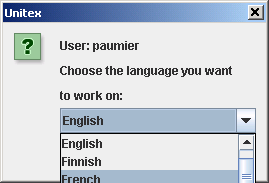
\includegraphics[width=6.2cm]{resources/img/fig2-1.png}
\caption{\label{fig-language-selection}Sélection de la langue au lancement d’Unitex}
\end{center}
\end{figure}


\section{Format des textes}
\label{section-conversion-texte-unicode}
\index{Format!des textes}
\index{Corpus|see{Texte}}
\index{Unicode}
Unitex manipule des textes Unicode. Unicode est un standard qui décrit un codage universel 
des caractères. Chaque caractère se voit attribuer un numéro unique, ce qui permet
de représenter des textes sans avoir à tenir compte des codages propres aux différentes 
machines et/ou systèmes d’exploitation. Unitex utilise une représentation codée sur deux 
octets du standard Unicode 3.0, appelée Unicode Little-Endian (pour plus de détails, voir
\cite{UNICODE}).

\bigskip
\index{Fichier!transcodage}
\noindent Les textes fournis avec Unitex sont déjà au format Unicode. Si vous essayez d’ouvrir un
texte qui n’est pas au format Unicode, le programme vous proposera de le convertir automatiquement 
(voir figure~\ref{auto-transcoding}). Cette conversion se base sur la langue courante : si vous
travaillez en français, Unitex vous proposera de convertir votre texte\footnote{Unitex propose
également de convertir automatiquement les graphes et dictionnaires qui ne sont pas en Unicode
Little-Endian.}, en supposant qu’il est codé avec un codage français. Par défaut, Unitex vous
propose soit de remplacer le texte original, soit de renommer le fichier d’origine en insérant
\verb$.old$ au début de son extension. Par exemple, si un fichier ASCII est nommé \verb$biniou.txt$,
le processus de conversion va créer une copie de ce fichier ASCII nommée \verb$biniou.old.txt$, et
va remplacer le contenu de \verb$biniou.txt$ par son équivalent en Unicode.

\begin{figure}[!h]
\begin{center}
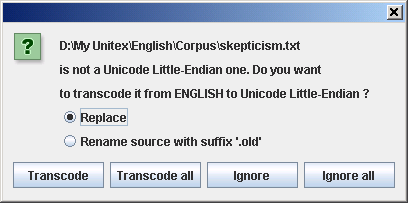
\includegraphics[width=10cm]{resources/img/fig2-2.png}
\caption{\label{auto-transcoding}Conversion automatique d’un texte non Unicode}
\end{center}
\end{figure}

\bigskip
\noindent Si le codage proposé par défaut n’est pas le bon, ou si vous voulez renommer le fichier
autrement qu’avec le suffixe \verb$.old$,vous pouvez utiliser la commande "Transcode Files"
dans le menu "File Edition". Cette commande vous permet de choisir les codages d’origine
et de destination des documents à convertir (voir figure~\ref{transcoding}). Par défaut, le codage
source proposé est celui qui correspond à la langue courante, et le codage de destination est
Unicode Little-Endian. Vous pouvez modifier ces choix, en sélectionnant n’importe quels
codages de source et destination. Ainsi, vous pouvez si vous le souhaitez convertir vos données
dans d’autres codages, comme par exemple UTF-8 si vous voulez en faire des pages
web. Le bouton "Add Files" vous permet de sélectionner les fichiers à convertir. Le bouton
"Remove Files" permet de retirer de la liste des fichiers sélectionnés par erreur. Le bouton
"Transcode" lancera la conversion de tous les fichiers. Si une erreur survient lors du traitement
d’un fichier (par exemple, un fichier qui serait déjà en Unicode), le traitement continue
avec le fichier suivant.


\begin{figure}[!h]
\begin{center}
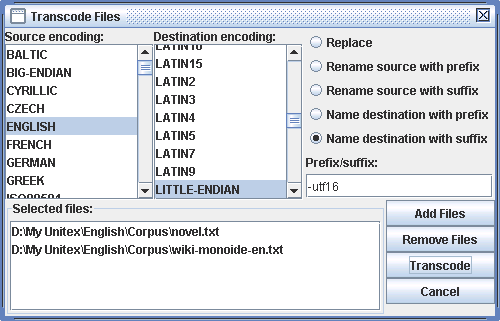
\includegraphics[width=12cm]{resources/img/fig2-3.png}
\caption{\label{transcoding}Conversion de fichiers}
\end{center}
\end{figure}

\noindent Pour obtenir du texte au bon format, vous pouvez également utiliser un traitement de
texte comme le logiciel libre OpenOffice.org (\cite{OpenOffice}) ou Microsoft Word, et sauvegarder
votre document au format "Texte unicode". Dans OpenOffice Writer, vous devez choisir le format
"Coded Text (*.txt)" puis le codage "Unicode" dans la fenêtre de configuration comme le montre la
figure~\ref{OfficeWriter}.

\begin{figure}[!h]
\begin{center}
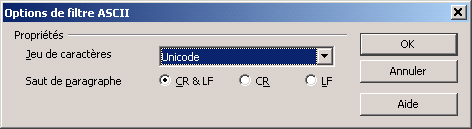
\includegraphics[width=12.5cm]{resources/img/fig2-4.png}
\caption{\label{OfficeWriter}Sauvegarde en Unicode dans OpenOffice Writer}
\end{center}
\end{figure}

\noindent Par défaut, le codage proposé sur un PC est toujours Unicode Little-Endian. Les textes 
ainsi obtenus ne contiennent plus d’informations de formatage (police, couleurs, etc.) et sont
prêts à être utilisés avec Unitex.

\bigskip
\noindent 
Vous pouvez choisir le codage par défaut, UTF16LE, UTF16BE ou UTF8 dans l'onglet, "Encoding" grâce
au sous-menu "Preference"  dans le menu "Info". Ce codage n'est valide que pour la langue
courante.

\begin{figure}[!h]
\begin{center}
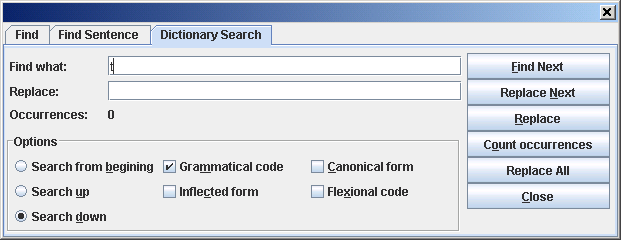
\includegraphics[width=10cm]{resources/img/fig2-5.png}
\caption{Choix de l'encodage par défaut pour la langue courante}
\end{center}
\end{figure}

% For small files...
\section{Édition de textes}
Vous avez également la possibilité d’utiliser l’éditeur de texte intégré à Unitex, accessible
via la commande "Open..." du menu "File Edition". Cet éditeur vous propose des fonctionnalités
de recherche et remplacement propres aux textes et dictionnaires manipulés par Unitex. Pour y
accéder, cliquez sur l’icône "Find" (jumelles). Vous verrez alors apparaître une fenêtre divisée en
trois onglets. L’onglet "Find" correspond aux opérations de recherche habituelles. Si vous ouvrez un
texte découpé en phrases, vous aurez la possibilité de faire une recherche par numéro de phrase dans
l’onglet "Find Sentence". Enfin, l’onglet "Dictionary Search", visible sur la
figure~\ref{dictionary-search}, vous permet d’effectuer des opérations propres aux dictionnaires
électroniques. En particulier, vous pouvez effectuer une recherche en spécifiant si elle doit porter
sur la forme fléchie, le lemme, les codes grammaticaux et sémantiques et/ou les codes flexionnels.
Ainsi, si vous voulez rechercher tous les verbes qui ont le trait sémantique
\verb$t$, marquant la transitivité, il vous suffit de chercher \verb$t$ en cochant
"Grammatical code". Vous obtiendrez ainsi les entrées voulues, sans ambiguïtés avec toutes les
autres occurrences de la lettre \verb$t$.


\begin{figure}[!h]
\begin{center}
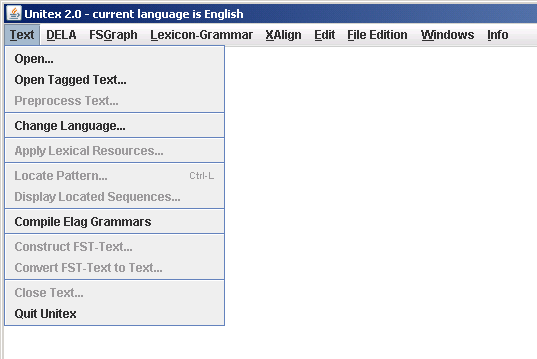
\includegraphics[width=15cm]{resources/img/fig2-6.png}
\caption{Recherche du trait sémantique \texttt{t}dans un dictionnaire
électronique\label{dictionary-search}}
\end{center}
\end{figure}


\section{Ouverture d’un texte}
\noindent Unitex propose d’ouvrir deux types de fichiers textes. \index{Fichier!texte}
Les fichiers portant l’extension \verb+.snt+ sont des fichiers textes prétraités 
par Unitex qui sont prêts à être manipulés par les différentes fonctions du système.
Les fichiers portant l’extension \verb+.txt+ sont des fichiers bruts.
Pour utiliser un texte, il faut donc commencer par ouvrir le fichier  \verb+.txt+
correspondant en cliquant sur "Open..." dans le menu "Text".


\begin{figure}[!h]
\begin{center}
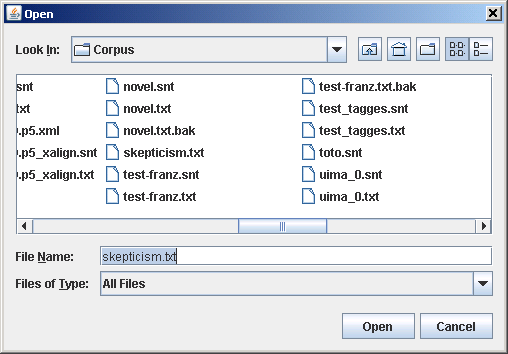
\includegraphics[width=14cm]{resources/img/fig2-7.png}
\caption{Menu Text}
\end{center}
\end{figure}

\begin{figure}[!h]
\begin{center}
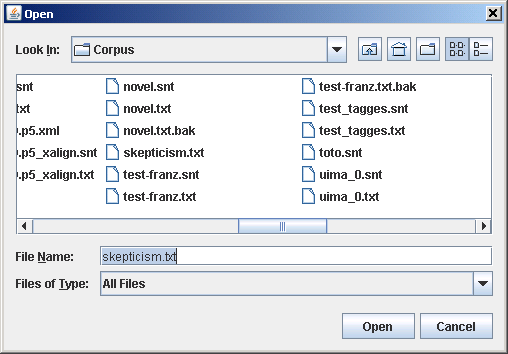
\includegraphics[width=13cm]{resources/img/fig2-8.png}
\caption{Ouverture d’un texte Unicode}
\end{center}
\end{figure}



\section{Prétraitement du texte}
\index{Texte!prétraitement}
\noindent Une fois le texte sélectionné, Unitex vous propose de le prétraiter. Le prétraitement du
texte consiste à lui appliquer les opérations suivantes : normalisation des séparateurs, 
découpage en unités lexicales, normalisation de formes non ambiguës, découpage en phrases
et application des dictionnaires. Si vous refusez le prétraitement, le texte sera néanmoins
normalisé et découpé en unités lexicales, car ces opérations sont indispensables au
fonctionnement d’Unitex. Il vous sera toujours possible d’effectuer le prétraitement plus tard,
en cliquant sur "Preprocess text..." dans le menu "Text".


\begin{figure}[!h]
\begin{center}
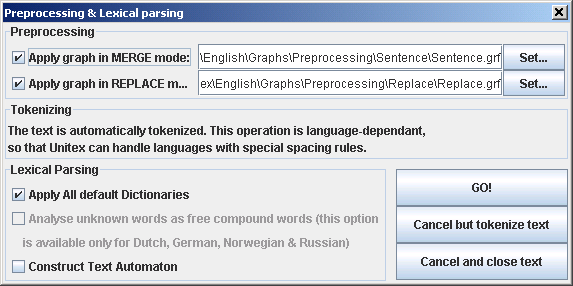
\includegraphics[width=15cm]{resources/img/fig2-9.png}
\caption{Fenêtre de prétraitement\label{fig-preprocessing-frame}}
\end{center}
\end{figure}

\bigskip
\noindent 
Si vous acceptez le prétraitement, Unitex vous proposera de le paramétrer grâce à la fenêtre de la
figure~\ref{fig-preprocessing-frame}. L’option "Apply FST2 in MERGE mode" sert à effectuer le
découpage du texte en phrases. L’option "Apply FST2 in REPLACE mode" est utilisée pour effectuer des
remplacements dans le texte, le plus souvent des normalisations de formes non ambiguës. L’option
"Apply All default Dictionaries" permet d’appliquer au texte des dictionnaires au format DELA
(Dictionnaires Electroniques du LADL). \index{DELA} L’option "Analyse unknown words as free 
compound words" est utilisée en norvégien pour analyser correctement les mots composés libres
formés par soudure de mots simples. Enfin, l’option "Construct Text Automaton" est utilisée
pour construire l’automate du texte. Cette option est désactivée par défaut, car elle entraîne
une forte consommation de mémoire et d’espace disque si le texte est trop volumineux. La
construction de l’automate du texte sera abordée dans le chapitre~\ref{chap-text-automaton}.

\bigskip
\noindent NOTE: si vous cliquez sur "Cancel but tokenize text", le programme effectuera malgré
tout la normalisation des séparateurs et le découpage en unités lexicales ; cliquez sur "Cancel
and close text" pour annuler complètement l’opération.


\subsection{Normalisation des séparateurs}
\index{Normalisation!des séparateurs}\index{Séparateurs de mots}\index{Texte!normalisation}
Les séparateurs usuels sont l’espace, la tabulation et le retour à la ligne. On peut rencontrer
plusieurs séparateurs consécutifs dans des textes, mais comme cela n’est d’aucune utilité
pour une analyse linguistique, on normalise ces séparateurs selon les règles suivantes:

\begin{itemize}
  \item toute suite de séparateurs contenant au moins un retour à la ligne est remplacée par
  un unique retour à la ligne
  \item toute autre suite de séparateurs est remplacée par un espace.
\end{itemize}

\bigskip
\noindent 
La distinction entre espace et retour à la ligne est conservée à cette étape car la présence
de retours à la ligne peut intervenir dans le découpage du texte en phrases. Le résultat de
la normalisation d’un fichier appelé \verb+mon_texte.txt+ est un fichier situé dans le même
répertoire que le \verb+.txt+ et dont le nom est \verb+mon_texte.snt+. \index{Fichier!\verb+.snt+}

\bigskip
\noindent NOTE: lorsque l’on prétraite un texte depuis l’interface graphique, un répertoire nommé

% do not remove this line jump 
\noindent \verb+mon_texte.snt+ est créé immédiatement après la normalisation. Ce répertoire, appelé
répertoire du texte, \index{Répertoire!du texte}
\index{Texte!répertoire du} contiendra toutes les données relatives à ce texte.



\subsection{Découpage en phrases}
\label{section-sentence-splitting}
\index{Découpage!en phrases}\index{Texte!découpage en phrases}
\index{Grammaires!découpage en phrases}
Le découpage en phrases est une étape importante du prétraitement car elle va permettre
de définir des unités de traitement linguistique. Ce découpage sera utilisé par le programme
de construction de l’automate du texte. Contrairement à ce que l’on pourrait penser, la re-
cherche des limites de phrases n’est pas un problème trivial. Considérons le texte suivant :


\bigskip
\textit{La famille a appelé le Dr. Martin en urgence.}

\bigskip \noindent Le point qui suit \textit{Dr} est suivi d’un mot commençant par une majuscule;
il pourrait donc être considéré comme un point de fin de phrase, ce qui serait faux. Afin d’éviter
les problèmes de ce genre, dus à des ambiguïtés des symboles de ponctuation, on utilise des
grammaires qui décrivent les différents contextes où peuvent apparaître les limites de phrases.
La figure~\ref{fig-example-sentence-splitting} montre un exemple de grammaire de découpage en
phrases.

\begin{figure}[!h]
\begin{center}
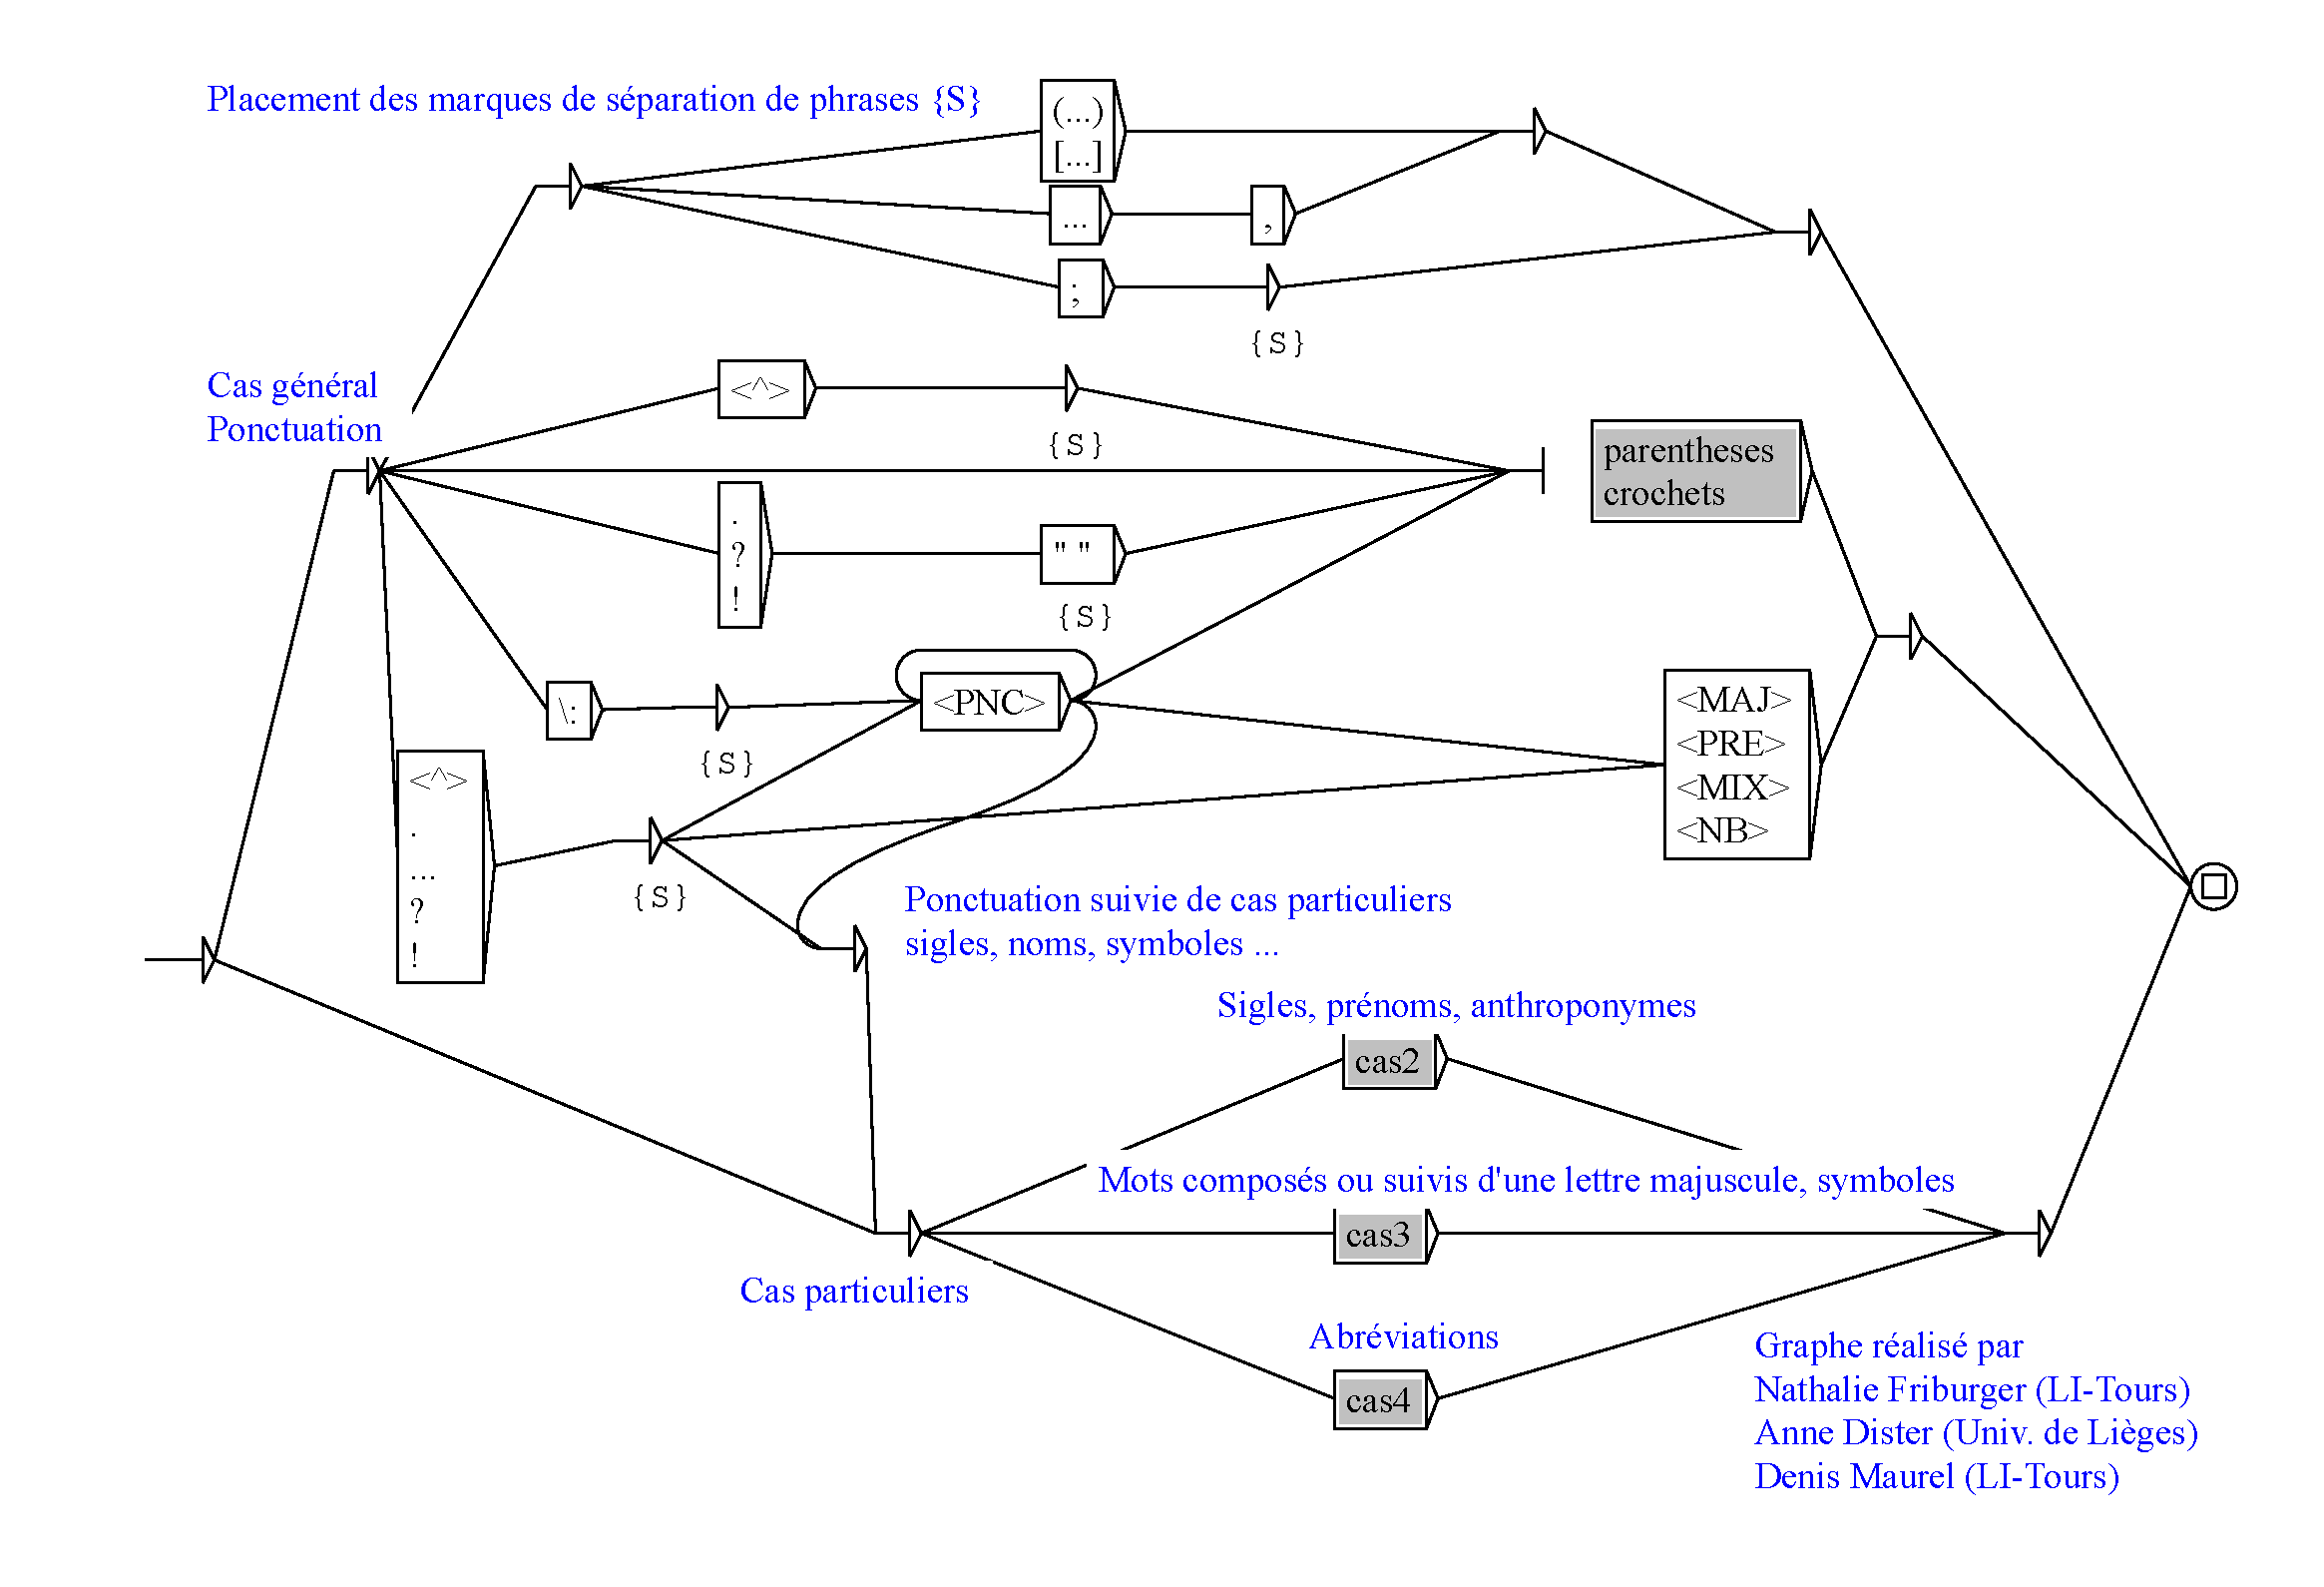
\includegraphics[width=15cm]{resources/img/fig2-10.pdf}
\caption{Grammaire de découpage en phrases pour le français
\label{fig-example-sentence-splitting}}
\end{center}
\end{figure}

\noindent  Lorsqu’un chemin de la grammaire reconnaît une séquence dans le texte et que ce chemin
produit le symbole délimiteur de phrases \verb+{S}+\index{\verb+{S}+}\index{Délimiteur de phrases},
on insère ce symbole dans le texte. Ainsi,
un chemin de la grammaire de la figure~\ref{fig-example-sentence-splitting} reconnaît la séquence
composée d’un point d’interrogation et d’un mot commençant par une majuscule et insère le symbole 
\verb+{S}+ entre le point d’interrogation et le mot suivant. Le texte suivant :


\bigskip
\textit{Quelle heure est-il ? Huit heures.}

\bigskip
\noindent deviendrait donc :

\bigskip
\textit{Quelle heure est-il ?\{S\} Huit heures.}

\bigskip
\noindent Une grammaire de découpage peut manipuler les symboles spéciaux, ou méta-symboles, suivants :

\index{\verb+<E>+}\index{Epsilon|see{<E>}}
\index{\verb+<MOT>+}\index{\verb+<MIN>+}\index{\verb+<MAJ>+}\index{\verb+<PRE>+}\index{\verb+<NB>+}
\index{\verb+<PNC>+}\index{\verb+<^>+}\index{\verb+#+}\index{\verb+<WORD>+}\index{\verb+<UPPER>+}\index{Méta-symboles}
\index{\verb+<LOWER>+}\index{\verb+<FIRST>+}
\begin{itemize}
  \item \verb+<E>+~: mot vide, ou epsilon. Reconnaît la séquence vide~;
  \item \verb+<WORD>+~: reconnaît n’importe quelle suite de lettres~;
  \item \verb+<LOWER>+~: reconnaît n’importe quelle suite de lettres minuscules~;
  \item \verb+<UPPER>+~: reconnaît n’importe quelle suite de lettres majuscules~;
  \item \verb+<FIRST>+~: reconnaît n’importe quelle suite de lettres commençant par une majuscule~;
  \item \verb+<NB>+~: reconnaît n’importe quelle suite de chiffres contigus (1234 est reconnu mais pas 1 234)~; 
  \item \verb+<PNC>+~: reconnaît les symboles de ponctuation ; , ! ? : ainsi que les points d’exclamation
  	  et d’interrogation inversés de l’espagnol et quelques signes de ponctuation asiatiques~;
  \item <\verb+^+>~: reconnaît un retour à la ligne~;
  \item \verb+#+~: interdit la présence de l’espace.
\end{itemize}

\noindent  Les anciens codes correspondant à \verb+<WORD>+, \verb+<LOWER>+, \verb+<UPPER>+ et \verb+<FIRST>+
 étaient respectivement \verb+<MOT>+, \verb+<MIN>+, \verb+<MAJ>+ et \verb+<PRE>+.
 Ils restent opérationnels afin de conserver la compatibilité descendante
 du système avec les graphes existants, mais ils sont maintenant dépréciés,
 c'est-à-dire qu'on recommande de les éviter dans les graphes conçus pour fonctionner avec les versions plus récentes\footnote{À partir de la version 3.1bêta, révision 4072 du 2 octobre 2015.},
pour ne pas faire augmenter inutilement le nombre de masques lexicaux en usage.

\bigskip
\noindent Par défaut, l’espace est facultatif entre deux boîtes. Si l’on veut interdire la présence
de ce séparateur, il faut utiliser le symbole spécial \verb+#+. À l’inverse, si vous souhaitez
forcer la présence de l’espace, vous devez utiliser la séquence \verb+" "+. Les lettres minuscules
et majuscules sont définies par un fichier alphabet\index{Fichier!alphabet}\index{Alphabet}
(voir chapitre~\ref{chap-file-formats}). Pour plus de détails sur les graphes,
voir le chapitre~\ref{chap-grammars}. Pour plus de détails sur le découpage d’un texte en phrases,
voir \cite{ameliorer-decoupage-en-phrases}. La grammaire utilisée se nomme \verb+Sentence.fst2+ et
se trouve dans le répertoire suivant:\index{Fichier!\verb+Sentence.fst2+}

\bigskip
\verb+/(répertoire personnel)/(langue)/Graphs/Preprocessing/Sentence+

\bigskip
\noindent L’application de cette grammaire à un texte s’effectue grâce au programme \verb+Fst2Txt+
\index{\verb+Fst2Txt+}\index{Programmes externes!\verb+Fst2Txt+} en mode MERGE.\index{MERGE} 
Cela signifie que les sorties produites par la grammaire, en l’occurrence le symbole \verb+{S}+,
sont insérées dans le texte. Ce programme prend en entrée un fichier \verb+.snt+ et le modifie.


\subsection{Normalisation de formes non ambiguës}
\index{Normalisation!de formes non ambiguës}
\index{Grammaires!normalisation!de formes non ambiguës}

Certaines formes présentes dans les textes peuvent être normalisées (par exemple, la séquence
française "\textit{l'on}" est équivalente à la forme "\textit{on}"). Chaque utilisateur peut donc
vouloir effectuer des remplacements en fonction de ses besoins. Toutefois, il faut faire
attention à ce que les formes normalisées soient non ambiguës, ou à ce que la disparition de
l’ambiguïté soit sans conséquence pour l’application recherchée.


\bigskip
\noindent Si l’on décide de remplacer la forme "\textit{audit}" par "\textit{à le-dit}",
 la phrase :

\bigskip
\textit{La cour a procédé à un audit des comptes de cette société.}

\bigskip
\noindent sera remplacée par la phrase incorrecte :

\bigskip
\textit{La cour a procédé à un à le-dit des comptes de cette société.}

\bigskip
\noindent Il faut donc être très prudent lorsque l’on manipule la grammaire de normalisation.
Il faut également faire attention aux espaces.
En effet, si l’on remplace "\textit{c’}" par "\textit{ce}" non suivi par un espace, la phrase :


\bigskip
\textit{Est-ce que c’était toi ?}

\bigskip
\noindent sera remplacée par la séquence incorrecte :

\bigskip
\textit{Est-ce que ce était toi ?}

%\bigskip
%\noindent To avoid this problem, one should explicitly insert a space,
%\textit{i.e.} replace "\textit{'re}" by "\textit{ are}".

\bigskip
\noindent Les symboles acceptés par les grammaires de normalisation sont les mêmes que ceux
autorisés dans les grammaires de découpage en phrases. La grammaire utilisée se nomme
\verb+Replace.fst2+ et se trouve dans le répertoire suivant :

\bigskip \verb+/(répertoire personnel)/(langue)/Graphs/Preprocessing/Replace+

\bigskip
\noindent Comme pour le découpage en phrases, cette grammaire est utilisée avec le programme
\verb+Fst2Txt+ \index{Programmes externes!\verb+Fst2Txt+}\index{\verb+Fst2Txt+}, mais cette fois en
mode REPLACE, ce qui signifie que les entrées reconnues par la grammaire sont remplacées par les
séquences produites par celle-ci. On peut voir sur la figure~\ref{fig-normalization-grammar} une
grammaire qui normalise des contractions verbales en anglais.

\begin{figure}[!p]
\begin{center}
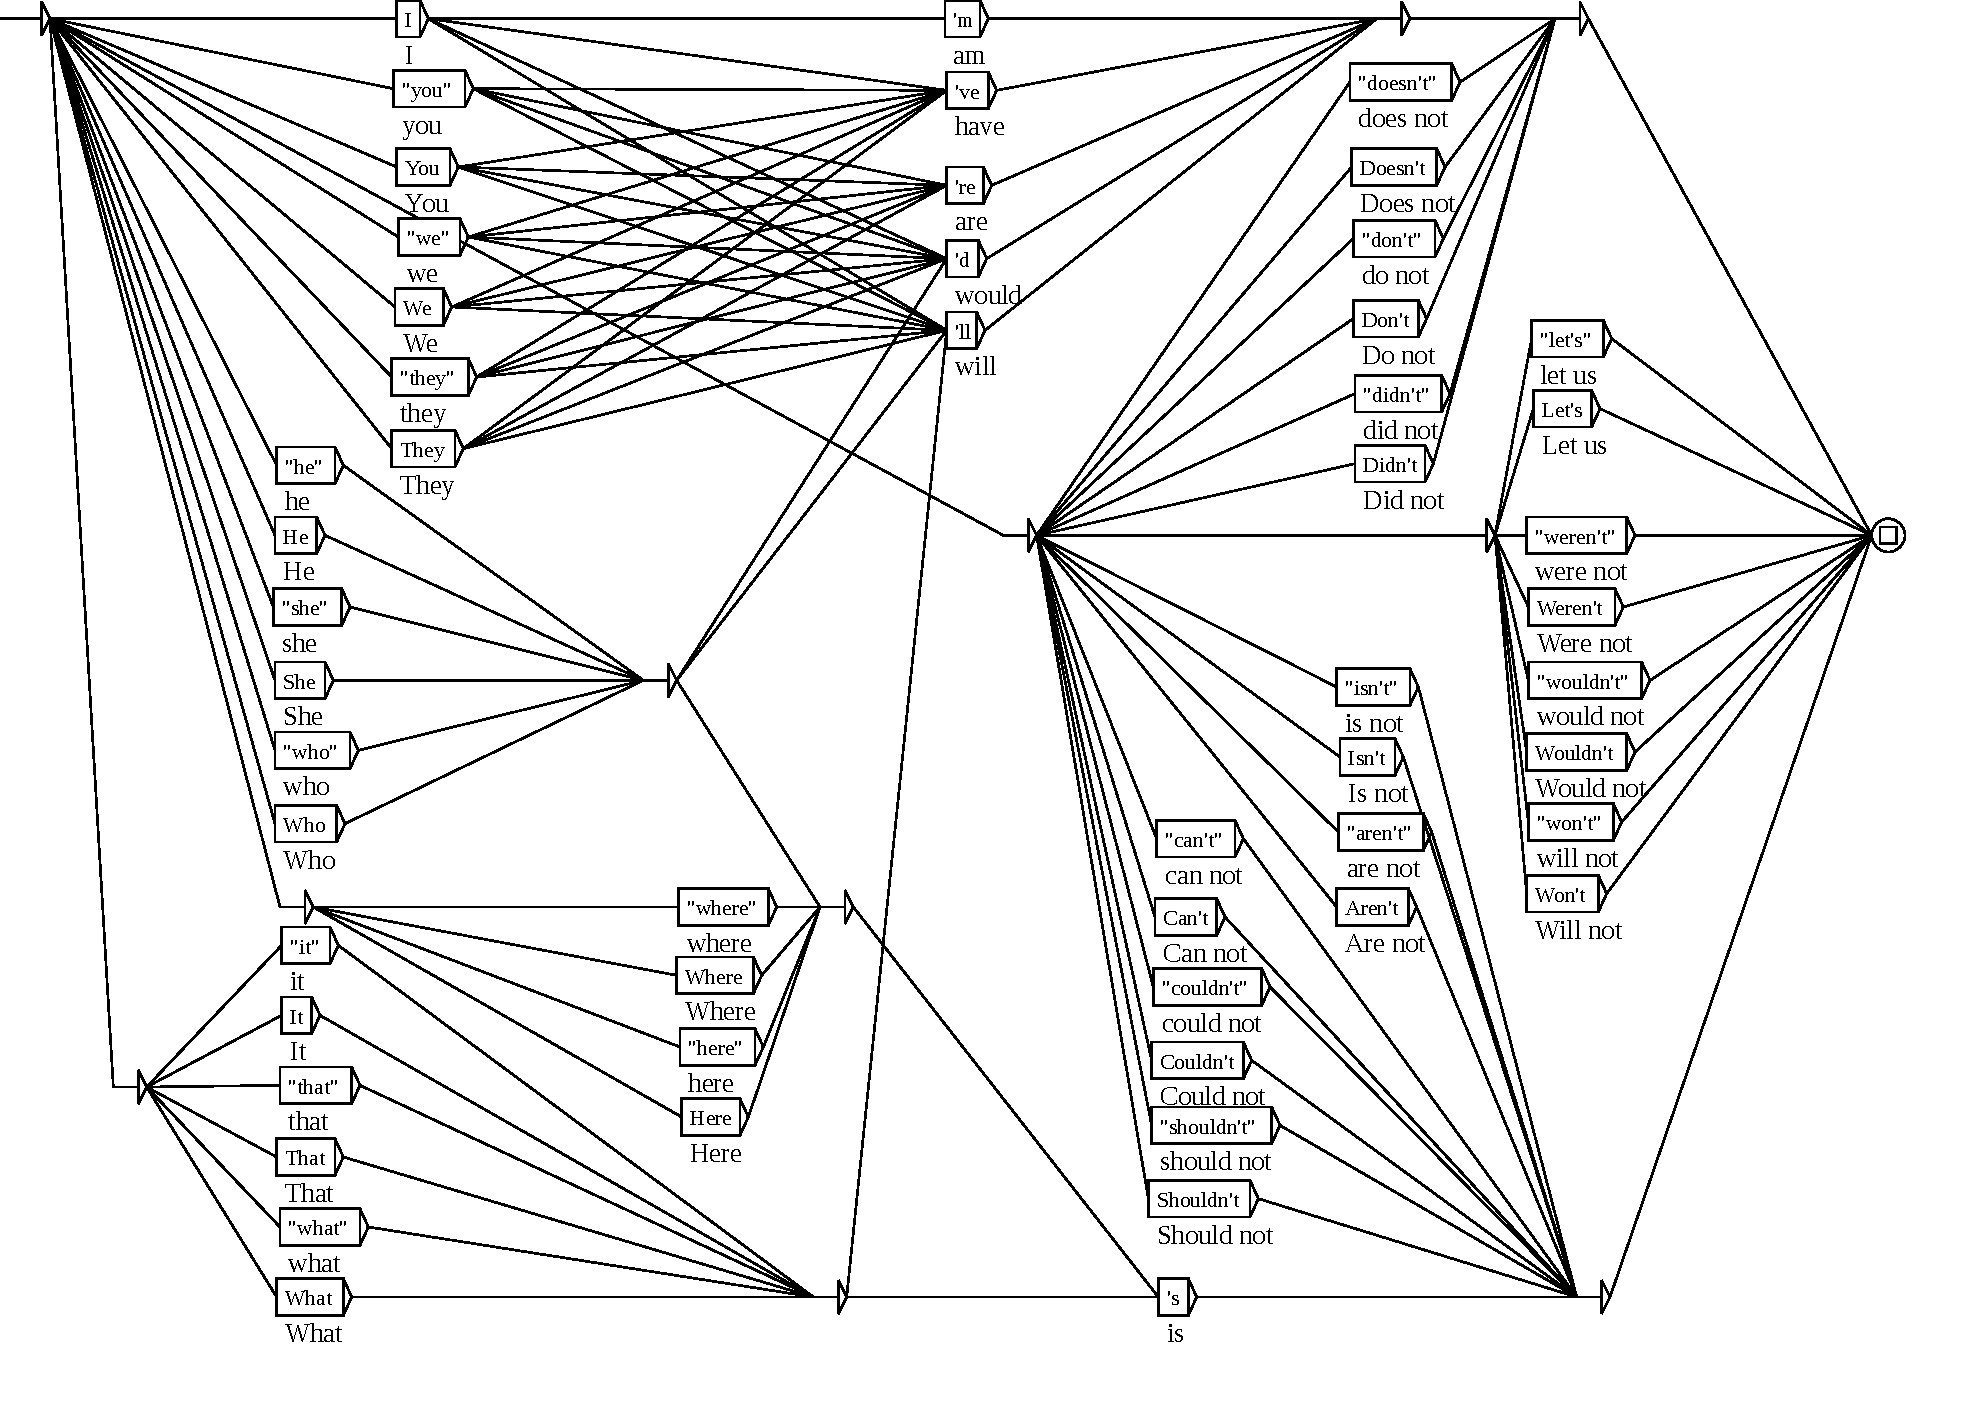
\includegraphics[height=17cm,angle=90]{resources/img/fig2-11.pdf}
\caption{Grammaire de normalisation de formes verbales en anglais\label{fig-normalization-grammar}}
\end{center}
\end{figure}



\subsection{Découpage du texte en unités lexicales}
\index{Texte!découpage en unités lexicales}
\index{Découpage!en unités lexicales}
\index{Token}\index{Tokenisation}
\label{tokenization}
Certaines langues, en particulier les langues asiatiques, utilisent les séparateurs de façon
différente des langues occidentales ; les espaces peuvent être interdits, facultatifs ou
obligatoires. Pour pouvoir gérer ces particularités au mieux, Unitex découpe les textes d’une
manière dépendante de la langue. Ainsi, les langues comme le français sont traitées selon le
principe suivant :

\bigskip
\noindent Une unité lexicale peut être :
\begin{itemize}
  \item soit le délimiteur de phrases \verb+{S}+;
  \item le marqueur \verb+{STOP}+.\index{\verb${STOP}$} Contrairement au délimiteur de phrases
  \verb+{S}+, le marqueur \verb+{STOP}+ ne peut JAMAIS être reconnu par une grammaire, de quelque
  façon que ce soit. Il peut être utilisé dans un corpus pour délimiter des élements. Par exemple,
  si un corpus est formé de nouvelles séparées par \verb+{STOP}+, il est impossible pour une
  grammaire de reconnaître une séquence qui chevauche la fin d'une nouvelle et le début de la
  suivante;
  \item une étiquette lexicale \verb+{aujourd'hui,.ADV}+;
  \item une séquence de lettres contiguës (les lettres sont définies dans le fichier alphabet de la
  langue);
  \index{Fichier!alphabet}
  \item un (et un seul) caractère différrent d'une lettre, i.e. tous les caractères non définis
  dans le fichier alphabet de la langue courante; s'il s'agit d'une newline, il est remplacé par un
  espace.
\end{itemize}

\bigskip
\noindent Pour les autres langues, le découpage est effectué caractère par caractère, à l’exception
du délimiteur de phrases \verb+{S}+ le marqueur \verb+{STOP}+ et des étiquettes lexicales. Ce
découpage basique garantit le fonctionnement d’Unitex, mais limite l’optimisation des opérations de
recherche de motifs.


\bigskip
\noindent Quel que soit le mode de découpage, les retours à la ligne présents
dans un texte sont remplacés par des espaces. Ce découpage est effectué par le programme
\verb+Tokenize+\index{\verb+Tokenize+} \index{Programmes externes!\verb+Tokenize+}.
Ce programme produit plusieurs fichiers, stockés dans le répertoire du texte :
\begin{itemize}
  \item \verb+tokens.txt+ contient la liste des unités lexicales dans l’ordre où elles ont été
  	  trouvées dans le texte;\index{Fichier!\verb+tokens.txt+}
  \item \verb+text.cod+  contient un tableau d’entiers; chaque entier correspondant à l’indice d’une
  	  unité lexicale dans le fichier \verb+tokens.txt+;
  \index{Fichier!\verb+text.cod+}
  \item \verb+tok_by_freq.txt+ contient la liste des unités lexicales triée par ordre de fréquence;
  \index{Fichier!\verb+tok_by_freq.txt+}
  \item \verb+tok_by_alph.txt+ contient la liste des unités lexicales triée par ordre alphabétique;
  \index{Fichier!\verb+tok_by_alph.txt+}
\item \verb+stats.n+ contient quelques statistiques sur le texte. \index{Fichier!\verb+stats.n+}
\end{itemize}

\bigskip
\noindent Le découpage du texte :

\bigskip
\textit{Un sou c’est un sou.}

\bigskip
\noindent donne la liste d’unités lexicales suivantes :  \textit{UN} ESPACE \textit{sou c ’ est un
.}

\bigskip
\noindent On peut remarquer qu’il est tenu compte de la casse (Un et un sont deux unités distinctes), mais que chaque unité n’est codée qu’une fois. En numérotant ces unités de 0 à 7,
ce texte peut être représenté par la séquence d’entiers décrite dans le tableau suivant :

\bigskip
\begin{table}[h]
\begin{center}
\begin{tabular}{|p{2.8cm}||c|c|c|c|c|c|c|c|c|c|c|c|}
\hline
Indice             & 0 & 1 & 2 & 1 & 3 & 1 & 4 & 1 & 2 & 5
\\
\hline
Unité lexicale correspondante & \textit{UN} &   & \textit{sou} &   & \textit{est} &  & \textit{UN}
& & \textit{sou} & \textit{.}
\\
\hline
\end{tabular}
\caption{Représentation du texte \textit{Un sou c’est un sou.}}
\end{center}
\end{table}

\bigskip
\noindent Pour plus de détails, voir le chapitre~\ref{chap-file-formats}.

\begin{figure}[!h]
\begin{center}
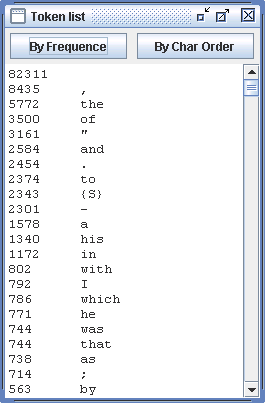
\includegraphics[height=10cm]{resources/img/fig2-12.png}
\caption{Unités lexicales d’un texte anglais triées par fréquence}
\end{center}
\end{figure}



\subsection{Application de dictionnaires}
\label{text-applying-dictionaries}
\index{Dictionnaire!application}
\index{Ressources!lexicales|see{Dictionnaire}}
L’application de dictionnaires consiste à construire le sous-ensemble des dictionnaires
ne contenant que les formes présentes dans le texte. Ainsi, le résultat de l’application des
dictionnaires du français au texte \textit{Igor mange une pomme de terre} produit le dictionnaire de
mots simples suivant :
\index{Mots!simples}

\bigskip
\begin{verbatim}
de,.DET+z1
de,.PREP+z1
de,.XI+z1
mange,manger.V+z1:P1s:P3s:S1s:S3s:Y2s
pomme,.A+z1:ms:fs:mp:fp
pomme,.N+z1:fs
pomme,pommer.V+z3:P1s:P3s:S1s:S3s:Y2s
terre,.N+z1:fs
terre,terrer.V+z1:P1s:P3s:S1s:S3s:Y2s
une,.N+z1:fs
une,un.DET+z1:fs
\end{verbatim}

\bigskip
\noindent ainsi que le dictionnaire de mots composés contenant l’unique entrée
:\index{Mots!composés}

\bigskip
\begin{verbatim}
pomme de terre,.N+z1:fs
\end{verbatim}

\bigskip
\noindent La séquence \textit{Igor} n'étant ni un mot simple du français, ni une partie de mot
composé, a été considérée comme un mot inconnu.\index{Mots!inconnus} L’application de dictionnaires
s’effectue avec le programme \verb+Dico+.\index{\verb+Dico+}\index{Programmes externes!\verb+Dico+}
Les trois fichiers produits (\verb+dlf+ pour les mots simples, \verb+dlc+ pour les mots composés et
\verb+err+ pour les mots inconnus) sont placés dans le répertoire du texte. On appelle dictionnaires
du texte les fichiers \verb+dlf+ et \verb+dlc+
\index{Dictionnaire!du texte}
\index{Fichier!\verb+dlf+}
\index{Fichier!\verb+dlc+}\index{Fichier!\verb+err+}

\bigskip
\noindent Une fois l’application des dictionnaires effectuée, Unitex présente par ordre alphabétique
les mots simples, composés et inconnus trouvés dans une fenêtre. La figure~\ref{fig-Dico-application-results} montre les résultats pour un texte anglais.

\begin{figure}[!ht]
\begin{center}
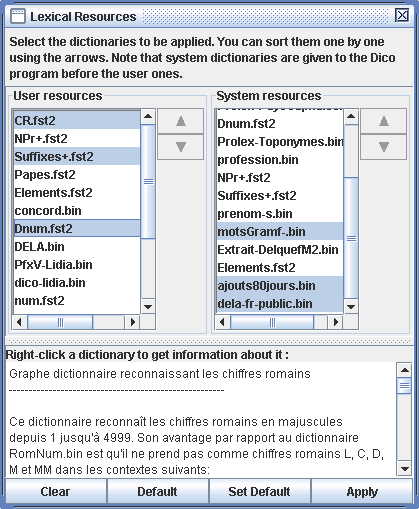
\includegraphics[width=12cm]{resources/img/fig2-13.png}
\caption{Résultats de l’application de dictionnaires sur un texte
anglais\label{fig-Dico-application-results}}
\end{center}
\end{figure}

\bigskip
\noindent Il est également possible d’appliquer des dictionnaires en dehors du prétraitement du
texte. Pour cela, il faut cliquer sur "Apply Lexical Resources..." dans le menu "Text". Unitex
affiche alors une fenêtre (voir figure ~\ref{fig-Dico-configuration}) qui permet de choisir la
liste des dictionnaires à appliquer.


\begin{figure}[!ht]
\begin{center}
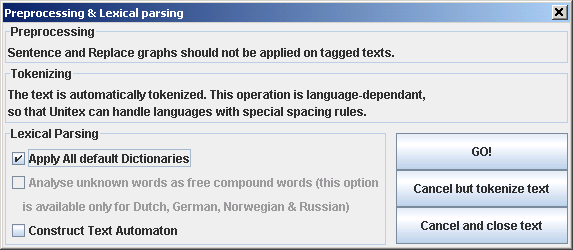
\includegraphics[width=10cm]{resources/img/fig2-14.png}
\caption{Paramétrage de l’application des dictionnaires\label{fig-Dico-configuration}}
\end{center}
\end{figure}

\bigskip
\noindent La liste "User resources" recense tous les dictionnaires \verb+.bin+ et \verb+.fst2+
présents dans le répertoire \verb+(langue)/Dela+ de l’utilisateur. Les dictionnaires du système sont
listés dans le cadre intitulé "System resources". Utilisez <Ctrl+click> pour sélectionner plusieurs
dictionnaires. Les dictionnaires systèmes sont appliqués avant les dictionnaires utilisateurs.
Vous pouvez choisir l'ordre des dictionnaires des listes utililisateur et système à l'aide des
flèches haut et bas (voir figure \ref{fig-Dico-configuration}). Le bouton "Set Default" vous permet
de définir la sélection courante de dictionnaires comme sélection par défaut. Cette sélection par
défaut sera utilisée lors du prétraitement si vous choisissez l’option "Apply All default
Dictionaries".\index{Dictionnaire!sélection par défaut}
Si vous effectuez un clic droit au-dessus d’un nom de dictionnaire, la documentation du
dictionnaire, si elle existe, s’affichera dans le cadre inférieur.


\subsection{Analyse des mots composés libres en néerlandais, allemand, norvégien et russe}
\index{Norvégien!mots composés libres}
\index{Allemand!mots composés libres}
\index{Néerlandais!mots composés libres}
\index{Russe!mots composés libres}
\index{Analyse des mots composés libres!langues germaniques}
\index{Mots!composés libres!langues germaniques}
\index{Analyse des mots composés libres!russe}
\index{Mots!composés libres!russe}

\label{section-Norwegian-compound-words}
Dans certaines langues comme le norvégien, il est possible de former des mots composés
libres en soudant leurs éléments. Par exemple, le mot \textit{aftenblad} signifiant \textit{journal
du soir} est obtenu en combinant les mots \textit{aften} (\textit{soir}) et \textit{blad}
(\textit{journal}). Le programme \verb+PolyLex+ \index{\verb+PolyLex+}\index{Programmes
externes!\verb+PolyLex+} explore la liste des mots inconnus après application des dictionnaires au
texte et essaye d’analyser chacun de ces mots comme un mot composé. Si un mot possède au moins une
analyse, il est retiré de la liste des mots inconnus et les lignes de dictionnaires produites pour
ce mot sont ajoutées au dictionnaire des mots simples du texte.

\section{Ouverture d’un texte taggué}
Un texte taggué est un texte contenant des entrées lexicales entre accolades comme par
exemple :


\bigskip
\textit{I do not like the \{square bracket,.N\} sign! \{S\}}

\bigskip
\noindent De tels tags permettent de lever des ambiguïtés en interdisant tout autre interprétation.
Dans notre exemple, on ne pourra pas reconnaître square bracket comme combinaison de deux mots
simples.


\bigskip
\noindent Toutefois, la présence de ces tags peut perturber l’application des graphes de
prétraitement. L’utilisateur dispose donc de la commande "Open Tagged Text..." dans le menu "Text",
grâce à laquelle il peut ouvrir un texte contenant des tags sans que les graphes de prétraitements
ne soient appliqués, comme on le voit sur la figure \ref{preprocess-tagged-text}.

\bigskip
\begin{figure}[!h]
\begin{center}
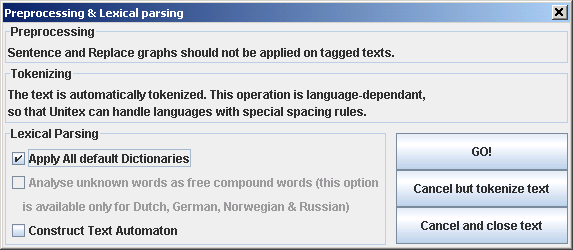
\includegraphics[width=14cm]{resources/img/fig2-15.png}
\caption{Prétraitement d’un texte taggué\label{preprocess-tagged-text}}
\end{center}
\end{figure}

